% Created 2018-01-29 月 03:08
% Intended LaTeX compiler: pdflatex
\documentclass{scrartcl}
    \usepackage{amsmath, amssymb, bm}
		\usepackage[utf8]{inputenc}
		\usepackage[dvipdfmx]{graphicx}
		\usepackage[dvipdfmx]{color}
		\usepackage[backend=biber,bibencoding=utf8]{biblatex}
		\usepackage{url}
		\usepackage{indentfirst}
		\usepackage[normalem]{ulem}
		\usepackage{longtable}
		\usepackage{minted}
		\usepackage{fancyvrb}
    \usepackage[dvipdfmx,colorlinks=false,pdfborder={0 0 0}]{hyperref}
    \usepackage{pxjahyper}
		\usepackage{biblatex}
\addbibresource{reference.bib}
\author{筑波大学情報学群情報科学類(201611350) 江畑 拓哉}
\date{\today}
\title{情報特別演習最終レポート}
\begin{document}

\maketitle
\tableofcontents


\section{概要}
\label{sec:orgaeb3230}
 今情報特別演習において私は、機械学習を初学者が学ぶための Web アプリ開発を行った。当初は大規模データベースを用いた機械学習APIを作るという目標であったが、特に機械学習を学んでいくにあたり、これの中身を理解するための初学者向けの解説の供給が少ないと感じたため、開発目標をやや変更した。\(\newline\)\\
 今回学習した内容は、\(\textcircled{\scriptsize1}\) 代表的な時系列分析の一つである(S)ARIMA モデル \(\textcircled{\scriptsize2}\) 大規模データベースの、特に時系列データベースの比較とその利用法 \(\textcircled{\scriptsize3}\) 更に機械学習等を実装する際に重要となる高速計算を JVM 言語内で行う手法 \(\textcircled{\scriptsize4}\) 開発言語として取り上げた Clojure/ClojureScript の、言語自体・これを用いたWeb開発手法、の4分野である。\\
 結果として ARIMA モデルとそれに付随する ADF 検定などを実装・解説を作成し、時系列データベースとして OpenTSDB を採用し設置した。更に JVM 上で高速計算を行うために、\(\href{http://jblas.org/}{jblas}\) や \(\href{https://software.intel.com/en-us/mkl}{Intel \textsuperscript{\textregistered} MATH \ KERNEL \  LIBRARY}\) を用いた GPU 演算 、 OpenCL の利用例を調べ比較し、一部を Web アプリの実装に活用した。そして \(\href{https://clojure.org/}{Clojure}\) という言語を身に着け、Clojure/ClojureScript を用いて JavaScript のライブラリである \(\href{https://reactjs.org/}{React.js}\) などを利用する手法についてまとめ、これらを利用してWebアプリの概形を実装した。\\

\section{序論}
\label{sec:orgb7fed70}
 この情報特別演習の初期テーマの決定はグループメンバーからの提案が元であった。その概要は、大規模データベースである \(\href{https://hbase.apache.org/}{Apache HBase \textsuperscript{\texttrademark}}\) (以降 ``HBase'' と呼称する) を用いて入力されたデータの因果関係を分析、予測する機械学習APIを作成するというものである。ここから因果関係と相関関係の違いについて学習し、機械学習手法について吟味した結果、ニューラルネットを用いた学習手法と、(S)ARIMA モデルを用いた時系列データ予測と Random Forest を用いた欠損値補完を組み合わせたものの2つの手法が議題に上がったが、後者を選択することになりこれを研究することになった。その中で機械学習を学ぶ際にその内部を知る必要があり、学んでいく際にその資料の供給が少ないことを感じ、その資料も兼ね備えたいと考え、また機械学習結果を視覚的にわかりやすく伝える目的も合わせて、Webアプリという形で開発を行うことに目標を定めた。\\
\newline\\
 機械学習という名前は世間に広く流布しており、それを用いたAPIとして例えば Microsoft Azure の \(\href{https://azure.microsoft.com/ja-jp/services/cognitive-services/computer-vision/}{Computer Vision API}\) 等を上げることができるが、この中身が解説されることはその必要性や機密性の問題から非常に少ない。またPythonやRといった言語に付属している統計処理、機械学習の関数などもその殆どが簡便化されており、例えば \(\href{https://www.rdocumentation.org/packages/forecast/versions/8.1/topics/auto.arima}{auto.arima()}\) 関数などはその中身を踏み込むことなく実行、モデルの比較を行うことができる。これは機械学習の利用者という立場からすれば素晴らしい進歩であると考えられるが、その反面機械学習を学ぶ立場になった場合、その中身を知らない状態でAPIや関数を利用することができるため、手放しに機械学習を理解できたと誤解してしまう可能性がある。\\
 このため主要な機械学習についてその中身を知ることができ、且つ理解ができるツールの作成は統計や機械学習を学びたいと志している、或いは先述のようなツールの中身について興味を持った者に対して、このWebアプリの開発は一定の需要があるのではないかと考えている。\\

\section{時系列データベースの比較と OpenTSDB の利用法}
\label{sec:org4cc369a}
 一般的に時系列データのような、単調増加する行キーを持つデータを通常の大規模データベースに保存することはデータの分散という点から問題が発生する。 \cite{hbase-reference} このため時系列データを扱うためのデータベースを考える必要がある。幸いなことに、初期案にあった HBase に対して時系列データを扱うことができるように拡張した \(\href{http://opentsdb.net/}{OpenTSDB}\) というデータベースがある。OpenTSDB は HTTP API として操作が許されており、また保存されているデータを確認することが容易であるように設計されている。今回は HBase を完全分散モードで利用する、というチームメンバーの目標に沿ってこちらのデータベースを採用した。\\
 他の時系列データベースの提案として考えられるものに、\(\textcircled{\scriptsize 1}\) \(\href{https://www.influxdata.com/}{InfluxDB}\) 、\(\textcircled{\scriptsize 2}\) \(\href{https://graphiteapp.org/}{Graphite}\) 、 \(\textcircled{\scriptsize 3}\) \(\href{https://www.datomic.com/}{Datomic}\) などを挙げることができる。\\

\subsection{InfluxDB}
\label{sec:org2e0dc1d}
 InfluxDB は InfluxData が開発を行っているデータベースであり、高機能なクラウドシステムを有料で使うことができるほか、オープンソースソフトウェアとしての利用も可能である。このデータベースの利点の一つに、利用方法が簡単であることが挙げられる。シングルノードでの利用に関してのみに焦点を絞れば、2017年12月において \(\href{https://www.archlinux.org/}{Arch\ Linux}\) でのインストールは、パッケージのインストールとサービスの起動の \href{https://wiki.archlinux.jp/index.php/InfluxDB}{2つのコマンド} で利用可能になる。またデータベースの読み書きに関しては、SQLに近い記法を用いた HTTP API を用いて行うことができ、今回の演習における開発言語である Clojure で必要な部分に関するラッパーを書くことは非常に簡単であった。また TICK stack と呼ばれる InfluxDB を含む時系列データを扱うための環境を追加でセットアップすればデータのモニタリング、収集、リアルタイム処理をより効率的に行うことができる。本演習の初期目標ではデータの入力をユーザが行うことができる設定になっていたため、悪意あるデータを監視することが容易であるという点、データベースの外側の分野までの広いサポート環境があるという点からこのデータベースは非常に魅力的である。\\
 このデータベースが扱うデータモデルの概要を以下に示す。\\
\begin{table}[htbp]
\caption{InfluxDB data model}
\centering
\begin{tabular}{|c|c|c|}
\hline
name(required) &  & \\
\hline
\hline
timestamp (required) & fields (required) & tags (optional)\\
\hline
 &  & \\
 &  & \\
 &  & \\
\vdots & \vdots & \vdots\\
\hline
\end{tabular}
\end{table}

 それぞれの用語についてその意味と例を挙げると以下のようになる。\\
\begin{itemize}
\item name データの名前 (ex. 日経平均株価)\\
 データの名前であり、何に関してのデータであるかを表す。\\
\item timestamp 時刻データ (ex. 2018-01-27T00:00:00Z)\\
 時刻データであり、いつのデータであるのかを示す。この場合の ``いつのデータ'' とは、データの登録日時ではなく、そのデータの発生日時である。\\
\item fields 測定値群 (ex. (終値:12000) (始値:11000))\\
 そのデータが持つ値を示す。いくつかの属性に従って複数の値を格納することができるが、ここに登録されるデータは索引付けされるべきものではないという点でタグ群と意味が異なる。\\
\item tags タグ群 (ex. (記録者:A) (ソース:東京株式市場))\\
 そのデータの持つ属性や追加情報を示す。ここに登録されるデータは索引付けさており、データの絞り込みを行う目的に用いられる。\\
\end{itemize}

\subsection{Graphite}
\label{sec:org2e5291a}
Graphite は Python を中心にして書かれた時系列データベースであり、同じく Python の Webフレームワークである Django と組み合わせることが、 Graphite 自身の Web UI コンポーネントが Django であるという点から非常に容易である。同時に Python は機械学習に関する API が豊富に存在しているため、本演習が純粋に ``Web APIの作成'' のみの目標であったならば当然こちらを用いて開発を行っていただろう。またデータベースの導入自体も Python のパッケージ管理システムである pip を用いて行うことができることから、純粋に Python によってすべての問題を解決することができる。更に Graphite のドキュメントは豊富に存在しており、例えば Monitoring with Graphite \cite{graphite-oreilly} を挙げることができる。\\
 Graphite の内部について簡単に説明を行うと、主に4つのコンポーネント、Carbon、Whisper、Cario、Djangoを中心に展開する。\\
\begin{itemize}
\item Carbon は、後述するデータベースそのものと言える Whisper に登録する役割を担っており、メトリクス\footnote[1]{metrics: 入手したデータを分析して数値化したもの}のバッファリングを行ったり他のデータベースにメトリクスをリレーさせたりすることができる。\\
\item Whisper は、入手したデータをファイルシステムに書き込み・読み出しを行う役割を担っており、この部分は Ceres と呼ばれるコンポーネントに置き換えることができる。両者の違いは、Whisper が保存領域を固定サイズとして確保するのに対して、Ceres は任意のサイズの保存領域を確保できるということにある。\\
\item Cario は、Graphite のグラフィックエンジンを担当しており、保存されているデータを視覚化する上で非常に重要な役割を果たしている。\\
\item Django は、Cario によって出力されたデータを表示する役割を担っており、データを扱う開発者はこの部分を見てデータを確認することになる。\\
\end{itemize}

 このデータベースが扱うデータモデルは階層構造を取っており、一例を紹介すると以下のようになる。\\
\begin{verse}
"stock\_price.nikkei\_index.close\_price 12000 1517055464"\\
\end{verse}
 上の文字列を送信することによって、 stock\_price の中の nikkei\_index の中にある close\_price という階層に 12000 という値を Unix 時間である 1517055464 のデータとして登録している。つまりこのデータは以下のようにな形に保存されたと考える。\\

\begin{figure}[htbp]
\centering
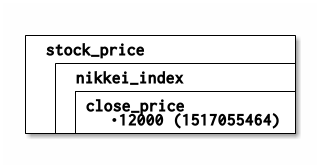
\includegraphics[width=8cm]{hoge.png}
\caption{Graphite example}
\end{figure}

\subsection{Datomic}
\label{sec:org3b07754}
  Datomic は他のデータベースとはかけ離れた設計が行われた新しい世代の分散型データベースである。 Clojure の作者である Rich Hickey 氏らが作成し、有料でメンテナンスとアップデートが付属されたクラウドシステムを使うことができる。また一年に限っては無料でこの機能を利用することもできる。これとは別に存在する無料版に関しては分散できるピア数などの制限がかかる。\\
  Datomic には2つの目標「情報を時間によって紐付け蓄積する」 「データベースアプリケーションのモデルをリモートアクセスするものからそれぞれのプログラムの中にあるものとする」\footnote{http://endot.org/notes/2014-01-10-using-datomic-with-riak/} がある。この考え方によって得られた大きな2つの特徴に、\textcircled{\scriptsize 1} Append-Only \textcircled{\scriptsize 2}データベースに独立したクエリーエンジンがある。\\
 Append-Onlyとはその名の通り、追加のみという意味で言い換えれば変更ができないということを意味する。これは情報を時間に紐付けることによって最新の情報を見ることができるため、情報を``書き換える''必要がなくなったためにできたことであり、トランザクション処理などのデータの管理を容易にすることができる。\\
 データベースに独立したクエリーエンジンとは、アプリケーション側でトランザクションやクエリ処理を実行するという意味を示しており、今まではデータベースに HTTP API などを用いてクエリを投げデータベース側がそのクエリを処理して結果を送信していたものをアプリケーション側に移すということになる。その意味で Datomic はアプリケーション側をピア \footnote{peer} と呼称する。\\
 ピアが扱うデータはデータベースではなくピア側のキャッシュに Read Only な形で LRU \footnote{Least Reacently Use}形式で保持される。データベースは書き込まれたデータを保存し、更新があればそれぞれのピアが持つデータベースに対して常に開いているノードに告知し、アプリケーション側から要求されるデータ群をそのまま返すことになる。これによってピア側のメモリキャッシュを貪欲に使うことができ、データベースのボトルネックを解消することができるようになっている。更にピア側のキャッシュ上のデータベースは実質ゼロコストで用いることができるため、 LRU が最適であるような目的のアプリケーションにこのデータベースを適用した場合データへのアクセスという点において他のデータベースに性能で劣ることはない。またクエリ処理を分散しているため、多くのクエリ処理をこなさなければならないピアが増えたとしてもキャッシュ上のデータを使っている限りはその処理によってデータベースに負荷がかかることもない。またデータベースの更新をピアに告知しなければならないという点でデータベースへの書き込みがネックになる可能性もあるが、これは論理的に分かれているデータごとにデータベースそのものを分割することで解決することができる。\\
 データベースのアクセス方法は Datalog と呼ばれる Clojure らしいシステムによって扱われるため、SQLに慣れている場合には苦労する可能性があるがアプリケーションに柔軟に組み込むことができる。これはデータがキャッシュ上に Read-Only な形で存在しているという特性と、 Clojrue が関数型言語の側面を持っているという点を考えれば、データベース上のデータを手元にあるデータであるかのように直に利用することができるということを意味している。また保存しているデータは必ず Datom という最小単位に分割されており、これを元にして様々な形にデータを変形することができる。\\
 このデータベースが扱うデータ例を以下に示す。\\

\begin{verse}
\{:nikkei-index/type ``close-price''\\
\hspace*{1em}:nikkei-index/value 12000\\
\hspace*{1em}:nikkei-index/timestamp 1517055464\}\\
\end{verse}
 データは nikkei-index/type に対する値として ``close-price'' が格納されている。nikkei-index に ``close-price'' が含まれているわけではない。\\

\begin{table}{h}
\caption{Datomicの特徴}
\centering
\begin{tabular}{|c|l|}
\hline
目指すもの & \(\cdot\) 情報は時間によって紐付ける\\
 & \(\cdot\) データベースアプリケーションのモデルをそれぞれのプログラム内に移動する\\
\hline
大きな特徴 & \(\cdot\) Append-Only データベース\\
 & \(\cdot\) データベース側ではなくアプリケーション側にクエリ処理エンジンがある\\
\hline
\end{tabular}
\end{table}

\begin{figure}[htbp]
\centering
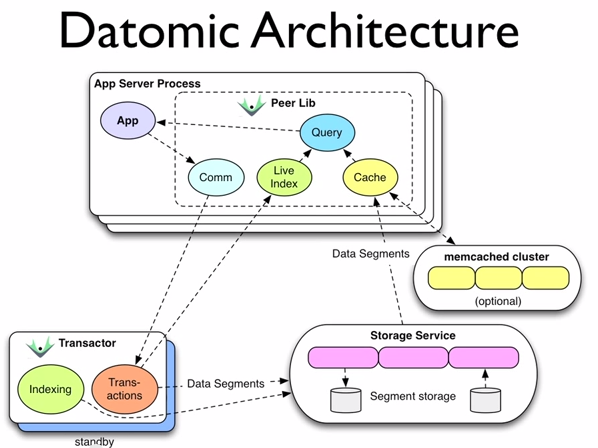
\includegraphics[width=15cm]{./datomic.png}
\caption{\href{http://endot.org/notes/2014-01-10-using-datomic-with-riak/datomic.png}{Talk Notes: Using Datomic With Riakより}}
\end{figure}

\newpage
\subsection{OpenTSDB}
\label{sec:orgcfc826f}
 OpenTSDB の特徴の説明、セットアップや利用方法に関して説明を行う前に、その基盤である HBase とその周辺知識について簡単にまとめ、その後 OpenTSDB についての説明を行う。\\

\subsubsection{HBase とその周辺知識}
\label{sec:orgb859c56}
 HBase とは \(\href{http://hadoop.apache.org/}{Apache \textsuperscript{\texttrademark} Hadoop \textsuperscript{\textregistered}}\) (以降 ``Hadoop'' と呼称する) と呼ばれる、大規模データの分散処理フレームワークのためのデータベースである。そして Hadoop の分散サービスを形成するために \(\href{http://zookeeper.apache.org/}{Apache \ Zookeeper \textsuperscript{\texttrademark}}\) (以降 ``Zookeeper'' と呼称する)という管理ツールが使われる。\\
\subsubsection{HBase}
\label{sec:orgde66049}
 HBase は NoSQL の一つである。NoSQL は大別して、\textcircled{\scriptsize 1}キーバリュー型\textcircled{\scriptsize 2}ワイドカラム型\textcircled{\scriptsize 3}ドキュメント型\textcircled{\scriptsize 4}グラフ型、があり HBase はワイドカラム型\footnote{簡単に説明するとデータを行ごとではなく列に対して管理しており特定の列を取り出して処理することに最適化されており、高いパフォーマンスやスケーラビリティを持っている。}に属している。\\

\begin{table}[htbp]
\caption{ワイドカラム型の例 (Name列を取り出すこと等を得意とする)}
\centering
\begin{tabular}{|c|c|c|c|c|}
\hline
ID & Name & Email & Birthday & Authorization\\
\hline
001 & Bob & bob @ foo.com & 1998/01/02 & true\\
002 & John & john @ bar.com & 1987/02/01 & false\\
\vdots & \vdots & \vdots & \vdots & \vdots\\
\hline
\end{tabular}
\end{table}

 Hadoop の HDFS (Hadoop Distributed File System) の補完を担っており、複数台のマシンのディスクを一台のディスクであるかのように扱うことができる。全体のデータは Region という単位で分割されており、これをそれぞれのディスクに1つ以上割り振っていくことで分散を行う。\\
 続いて HBase の論理データモデルについて説明を行う。最上位概念は Namespace と呼ばれるもので、この中には Table と呼ばれるデータを表形式で保持している概念を1個以上含んでいる。 一つ以上の RowKey 、一つ以上の ColumnFamily で構成されている。そして ColumnFamily には一つ以上の ColumnQualifier が存在している。行キーである ColumnQualifier と列キーである RowKey の交差点にはそれぞれ Cell と呼ばれる領域があり、ここにデータが格納されることになる。データは Timestamp とともに保存されており、 Cell にはそのデータが重ねて保存される。つまり Cell には Timestamp に紐付けられたデータが複数存在することになる。また、ワイドカラム型であるという特性上、Table は Rowkey でソートされた状態で保存されることになる。\\
 HBase の物理モデルの Table の構造はキーバリュー形式で保存されている。物理モデルの詳細はデータの分散などの説明も必要となるが、これ以上の内容は本演習で理解することができなかったため説明を省略する。\\

\begin{figure}[htbp]
\centering
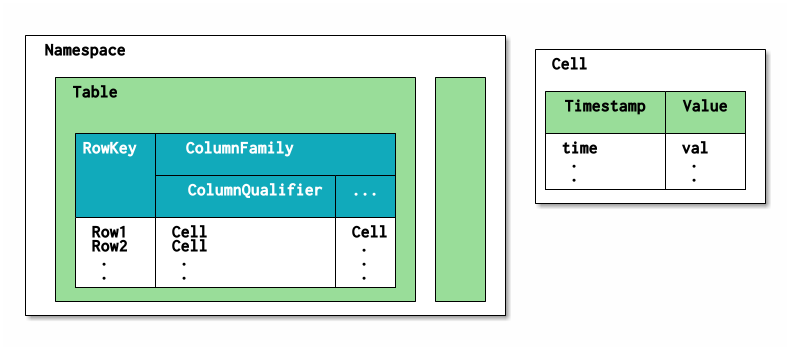
\includegraphics[width=.9\linewidth]{hoge2.png}
\caption{HBase の論理データモデル}
\end{figure}

\subsubsection{Hadoop}
\label{sec:orge829be6}
 Hadoop は大規模データセットの分散処理フレームワークである。 Hadoop はモジュール化されているため、そのコンポーネントの殆どを別のソフトウェアに入れ替えることもできる柔軟な設計がされている。今演習では標準的な Hadoop の構成に付随してインストールされる、\textcircled{\scriptsize 1}Hadoop Common \textcircled{\scriptsize 2}Hadoop YARN\footnote{Yet Another Resource Negotiator} \textcircled{\scriptsize 3}Hadoop MapReduce \textcircled{\scriptsize 4}Hadoop Distributed File System (HDFS) をそのまま利用している。\\
 Common は他のモジュールに利用される基本的なライブラリ群である。 YARN は Hadoop のリソース管理やスケジューリングを行い、 MapReduce は分散処理のためのフレームワークである。 HDFS は分散ファイルシステムで、大容量ファイルを扱うことができる。HDFS は大量の小さなデータを高速に扱うことを不得手としているので、HBase がこの補完を行っている。\\
\subsubsection{Zookeeper}
\label{sec:org28b3083}
 Zookeeper は Hadoop などにおける、構成情報の管理、分散処理の提供、またグループサービスの提供なども行う、分散アプリケーション全体を管理するツールである。使用用途は多岐にわたり、例えば Hadoop などにおける構成管理、 \href{http://storm.apache.org/}{Apache Storm}\textsuperscript{\texttrademark} \footnote{リアルタイム高速分散処理フレームワーク} における処理の同期などに用いられる。ツリー状の階層化された名前空間を持ち、ノードと呼ばれる要素にサーバなどを割り当てている。高速処理や高い信頼性があるにもかかわらず、非常に簡単な API を持っていることが特徴である。ベンチマークとしては \href{http://zookeeper.apache.org/doc/current/zookeeperOver.html#fg_zkPerfRW}{Zookeeper\ 3.4\ Documentation} に記載されている。\\


\begin{figure}[htbp]
\centering
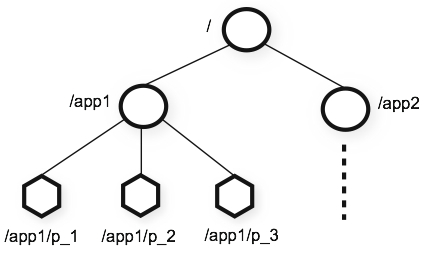
\includegraphics[width=8cm]{./zknamespace.jpg}
\caption{\href{http://zookeeper.apache.org/doc/current/zookeeperOver.html\#fg_zkPerfRW}{Zookeeperの階層構造}}
\end{figure}

\newline\\

\subsubsection{OpenTSDB}
\label{sec:org5769aaa}
 OpenTSDB とは HBase をホストとした \(\footnote {正確には Google の \href {https://cloud.google.com/bigtable/}{BigTable} もホストとなりうる}\) 時系列データベースで、その構成は\textcircled{\scriptsize 1} 時系列デーモン(以降 TSD と呼称する) \textcircled{\scriptsize 2} コマンドラインユーティリティ、の2つである。特徴としては TSD にマスター・スレーブといった上下関係がないこと、HBase などのホストに各アプリケーションが直接触れる必要がないこと、標準的に保存されているデータをブラウザから視覚的に確認することができることなどが挙げられる。\\
 これによって得られる恩恵として、アプリケーションをチームで開発・維持する際に OpenTSDB を軸にしてデータベース側とアプリケーション側に分割することができるということが考えられる。例えばアプリケーション側はデータベース側の分散等の開発が終わる前に仮設置の HBase に対して OpenTSDB を適用し、アプリケーションをほぼ本環境と同じように動かすことができる。またデータベースの分散数を増やしたい場合は、データベース側にのみ視点を当てて変更を行うことができる。\\

\begin{figure}[htbp]
\centering
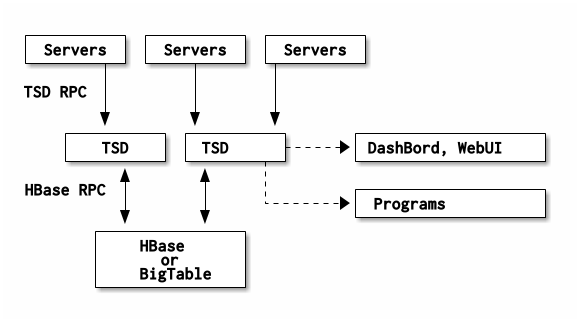
\includegraphics[width=10cm]{hoge3.png}
\caption{OpenTSDB の概略図}
\end{figure}

\newpage\\

 OpenTSDB の論理モデルは Metric と呼ばれるその時系列データのタイトルとも言える概念が最も外側に位置しており、この中にテーブルに近い構造が一つ含まれていると考えることが出来る。このテーブルの行キーはソートされたタイムスタンプであり、時系列データベースの要である。テーブルの列キーはタグと呼ばれるキーバリュー形式の識別子が0以上割り当てられており、これによって欲しいデータの絞り込みを行うことができる。\\

\begin{figure}[htbp]
\centering
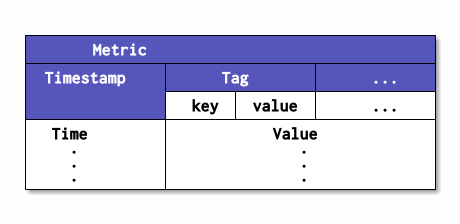
\includegraphics[width=12cm]{hoge4.png}
\caption{OpenTSDB の論理モデル}
\end{figure}

 OpenTSDB はそのアクセスを HTTP API を用いて行うことができる。以降にその概要をまとめる。\\

\subsubsection{OpenTSDB の HTTP API}
\label{sec:org8b12601}
 OpenTSDB を利用するにあたって重要な要素に HTTP API の習得がある。このクエリによってアプリケーション開発者はデータの取得や送信を行うことになる。尚、HTTP API を使わずに Telnet を用いる手段もあるが、どちらも機能として同等であるためここでは HTTP API についての説明のみに留める。\\
 API は、データの取得に関してはクエリ文字列とボディ部の両方の手段をサポートしており、ボディ部を用いる場合はクエリ文字列を用いるよりも詳細な検索をかけることが出来る。対してデータの送信は PUT メソッドによるボディ部を用いた手段のみが利用できる。 それぞれの具体例を示すと以下のようになる。\\

\begin{table}[htbp]
\caption{OpenTSDBにおけるクエリ例\textcircled{\scriptsize 1}}
\centering
\begin{tabular}{|c|l|}
\hline
前提条件 & \(\cdot\) http: //localhost:4242 に対して OpenTSDB が開いている\\
クエリ内容 & 1年前から現在までの Metric nikkei-index における\\
 &  タグについてkeyが ``type'' 、valueが ``close-price''\\
 &  であるデータを要求する\\
\hline
クエリ文字列 & \(\cdot\) http: //localhost:4242/api/query $\backslash$\\
 &  ?start=1y-ago\&m=avg:nikkei-index\{type=close\_price\}\\
\hline
ボディコンテンツ & \(\cdot\) http: //localhost:4242/api/query\\
 & \(\cdot\) Content-Type JSON\\
 & \(\cdot\) Body\\
 & \{ "start" : 1y-ago,\\
 &  "queries" :\\
 &   [\{"aggregator" : "sum",\\
 &      "metric" : "nikkei-index",\\
 &       "tags" :\\
 &        \{"type" : "close-price"\}\\
 &  \}]\\
 & \}\\
\hline
\end{tabular}
\end{table}

\begin{table}[htbp]
\caption{OpenTSDBにおけるクエリ例\textcircled{\scriptsize 2}}
\centering
\begin{tabular}{|c|l|}
\hline
前提条件 & \(\cdot\) http: //localhost:4242 に対して OpenTSDB が開いている\\
クエリ内容 & \(\cdot\) Metric ``nikkei-index'' の、\\
 &  タグが、key は``type''、value は``close-price'' である\\
 &  UnixTime が 1517055464 である時間に、\\
 &  12000 という値を保存する\\
\hline
 & \(\cdot\) http: //localhost:4242/api/put\\
 & \(\cdot\) Content-Type JSON\\
 & \(\cdot\) Body\\
 & \{ "metric" : "nikkei-index",\\
 &  "timestamp" : 1717055464,\\
 &  "value" : 12000,\\
 &  "tags" :\\
 &    \{"type" : "close-price"\}\\
 & \}\\
\hline
\end{tabular}
\end{table}

\section{Clojure を用いた JVM における高速計算技法}
\label{sec:org4a688e5}
\section{ARIMA モデルによる時系列分析}
\label{sec:orgd9a3128}
\section{Clojure/ClojureScript を用いた Web 開発}
\label{sec:org91eb446}
\section{MKKL の開発}
\label{sec:orgdea6be4}
\section{まとめと今後の課題}
\label{sec:orgada68fb}

\printbibliography\\
\end{document}
